\chapter{Implementation}
\label{chap:implementation}
This chapter shows the technical implementation of the ResNet-\gls{bilstm}-Attention framework by \textcite{Fischer2025ResNetBiLSTM} through translating the conceptual framework from \autoref{chap:methodology} into a functional system that processes manufacturing \gls{ocel}, extracts relevant features, trains models, and evaluates the fidelity of \gls{sbdt}.

\section{Architecture and System Setup}

\subsection{Architecture}
The implementation follows a modular architecture. It can process both streams and batches of manufacturing data.

\begin{figure}[htbp]
  \centering
  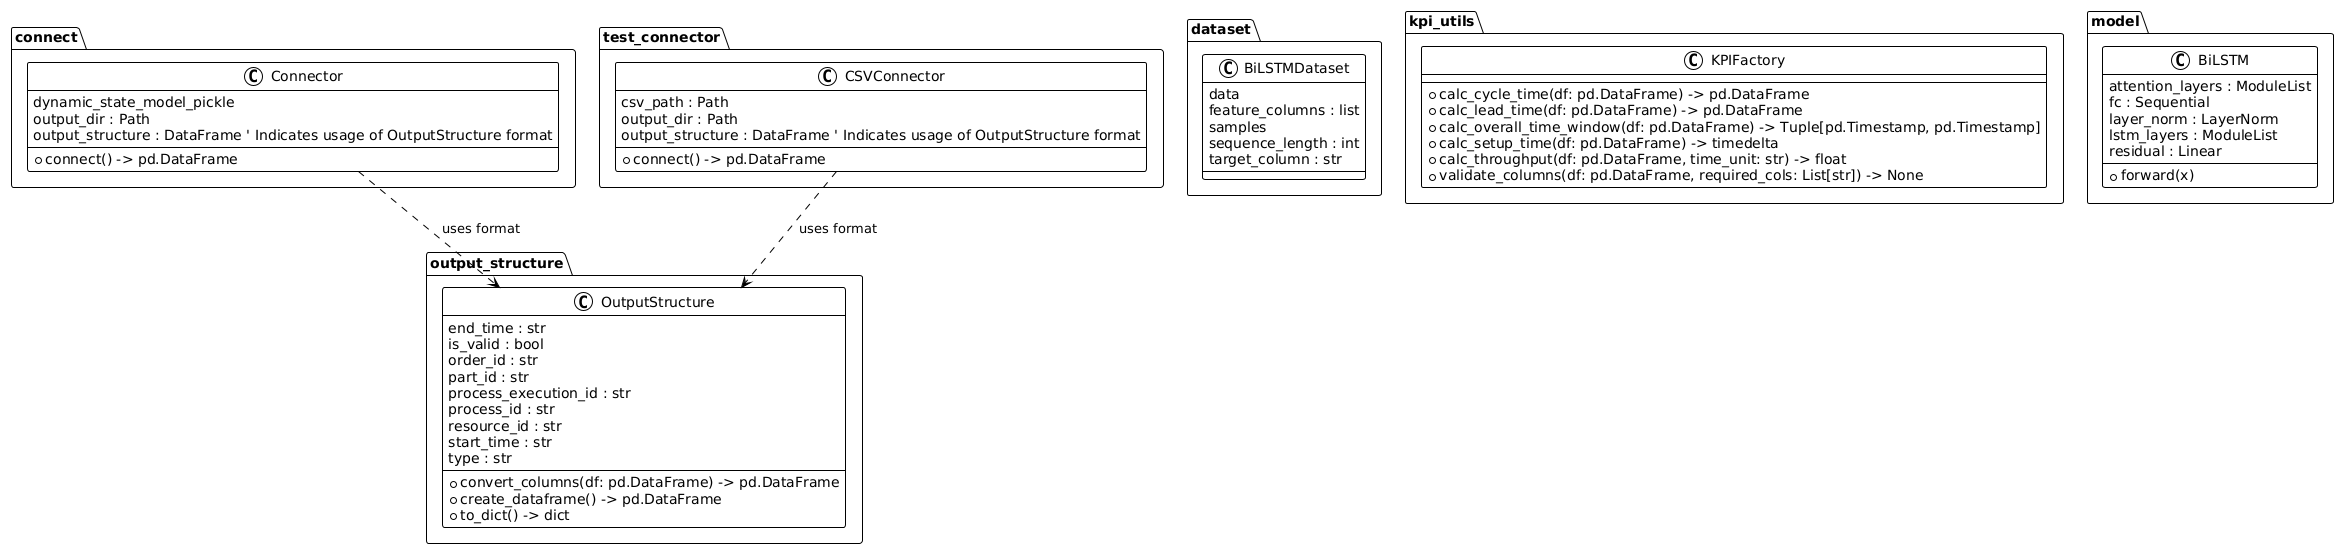
\includegraphics[width=1\textwidth]{figures/code.png}
  \caption[UML Diagram of the Implementation]{Unified Modelling Language (\gls{uml}) diagram of the ResNet-\gls{bilstm}-Attention framework for validating \gls{sbdt} in manufacturing environments.}
  \caption*{Source: Own illustration.}
  \label{fig:uml-diagram}
\end{figure}

The \gls{uml} model \autocite{PlantUML} in \autoref{fig:uml-diagram} illustrates the systems architecture, which consists of several components that interact to achieve the validation of \gls{sbdt}. The components include:
\begin{itemize}
  \item \textbf{Data Connectors:} In the given code, two classes \texttt{InputStructure} and \texttt{OutputStructure} are responsible for reading and writing data. The \texttt{InputStructure} class reads raw data from the twin simulation, while the \texttt{OutputStructure} class writes the processed data into the \gls{ocel} format developed for this framework, see \autoref{sec:event_log_processing}. The connector assigns IDs by enumeration for different parts, resources, and processes. The IDs are used to identify the different components in the manufacturing process. This is a requirement for \gls{oced}. The mapping is returned as JSON files for each category, respectively.
  \item \textbf{KPIFactory:} Contains utility functions to calculate a diverse set of \gls{kpi}s for \gls{ppc} evaluation of the process.
  \item \textbf{Baseline Model:} Implements a baseline model for comparison with the ResNet-\gls{bilstm}-Attention model. This model serves as a reference point to evaluate the performance of the more complex architecture.
  \item \textbf{PyTorch DataSet and DataLoader:} Handles the conversion of raw data into a format suitable for the ResNet-\gls{bilstm}-Attention model.
  \item \textbf{ResNet-\gls{bilstm}-Attention:} The core model that combines ResNet and \gls{bilstm} architectures with attention mechanisms to learn from the data.
\end{itemize}

\subsection{Tech Stack and Setup}
The implementation is built with Python 3.12 \autocite{Python}, using the following frameworks and libraries:

\begin{itemize}
  \item \textbf{PyTorch:} Powers the deep learning components, chosen for its dynamic computational graph that supports complex architecture development and debugging \autocite{PyTorch}.
  \item \textbf{Pandas \& NumPy:} Handle data manipulation, transformation, and numerical operations \autocite{NumPy, Pandas}.
  \item \textbf{Scikit-Learn:} Provides implementation of the baseline model and evaluation metrics \autocite{Scikit-Learn}.
  \item \textbf{Matplotlib \& Graphviz:} Generate visualizations of model architecture and performance \autocite{Matplotlib, Graphviz}.
  \item \textbf{UV Package Manager:} Ensures reproducible dependency management with exact version pinning \autocite{UV}.
\end{itemize}

PyTorch was preferred over TensorFlow due to its flexibility and ease of use, especially for research purposes. The implementation is designed to be modular and extensible, allowing for future enhancements and adaptations to different manufacturing environments.
The system is designed to run on a standard workstation with a multi-core CPU and an optional GPU for accelerated training. The given framework utilizes CUDA \autocite{NVIDIA_CUDA} for GPU acceleration.

\section*{Data Preprocessing}
\label{sec:event_log_processing}

After laying out the architecture and system setup, this section focuses on the data preprocessing steps necessary for preparing the input data for the baseline model.

\subsection{OCEL Format}

Both models used in this thesis require the input data to be in the \gls{ocel} format, see \autoref{sec:object-centric-event-logs}. The columns are inspired by the \gls{sbdt} comparison model by \textcite{schwede2024learning}. For the given framework, the format is expected as input in the following format:

\begin{table}[htbp]
  \centering
  \caption[Illustrative Manufacturing OCEL]{Detailed structure, data types, and description of the processed manufacturing \gls{ocel}.}
  \label{tab:output-structure-detailed}
  \begin{tabular}{l l p{6cm}} % l=left-aligned, p{width}=paragraph column
    \toprule
    \textbf{Column Name}            & \textbf{Data Type}       & \textbf{Description}                                                                                             \\
    \midrule
    \texttt{process\_execution\_id} & \texttt{int}             & Unique identifier for the specific process recorded.                                                             \\
    \texttt{order\_id}              & \texttt{Index (int/str)} & Identifier for the overall manufacturing order this event belongs to.                                            \\
    \texttt{start\_time}            & \texttt{Timestamp [UTC]} & The precise timestamp marking the beginning of the event, adjusted to UTC.                                       \\
    \texttt{end\_time}              & \texttt{Timestamp [UTC]} & The precise timestamp marking the end of the event, adjusted to UTC.                                             \\
    \texttt{duration}               & \texttt{float} (seconds) & The calculated duration of the event (\texttt{end\_time} - \texttt{start\_time}) in total seconds.               \\
    \texttt{part\_id}               & \texttt{int}             & Identifier for the specific part or component being processed or handled during the event.                       \\
    \texttt{resource\_id}           & \texttt{int}             & Identifier for the machine, station, or other resource involved in the event.                                    \\
    \texttt{process\_id}            & \texttt{int}             & Identifier indicating the type of process step or operation performed (e.g., milling, assembly).                 \\
    \texttt{type}                   & \texttt{str}             & A textual description or category classifying the type of data recorded.                                         \\
    \texttt{is\_valid}              & \texttt{bool}            & Boolean flag indicating whether the recorded event sequence or outcome is considered valid in the given setting. \\
    \bottomrule
  \end{tabular}
  \caption*{Source: Own tabulation.}
\end{table}

The terms are consistent with the upper cited framework. For the model components, following features may be considered:

\begin{enumerate}
  \item \textbf{Time Model:} \texttt{duration}, \texttt{sequence\_number}, \texttt{hour\_of\_day\_cos}, \texttt{hour\_of\_day\_sin}, \texttt{day\_of\_week\_cos}, \texttt{day\_of\_week\_sin}, \texttt{is\_break}, \texttt{is\_not\_weekday}.

  \item \textbf{Transition Model:} \texttt{part\_id}, \texttt{resource\_id}, \texttt{sequence\_number}, \texttt{duration}.

  \item \textbf{Transformation Model:} \texttt{part\_id}, \texttt{process\_id}, \texttt{sequence\_number}.

  \item \textbf{Quality Model:} Exclusion of quality information in the given model.

  \item \textbf{Resource Model:} \texttt{resource\_id}, \texttt{part\_id}, \texttt{process\_id}.

  \item \textbf{Resource Capacity Model:} \texttt{resource\_id}; Note: Insufficient data available for detailed capacity modelling.

  \item \textbf{Process Model:} \texttt{process\_id}, \texttt{duration}, \texttt{sequence\_number}.

  \item \textbf{\gls{kpi}-based Features:} \texttt{throughput}, \texttt{cycle\_time\_sec}, \texttt{lead\_time\_sec}, \texttt{setup\_time\_sec}.
\end{enumerate}

This table does not forbid adding relational logic by the modeller. For example, each ID may be a foreign key to another table. Each row in the \gls{ocel} represents a single event instance. This schema aligns with \gls{oced} principles (\autoref{sec:object-centric-event-logs}) by explicitly linking each recorded event instance (\texttt{process\_execution\_id} per timestamp) to the multiple object instances (\texttt{order\_id}, \texttt{part\_id}, \texttt{resource\_id}, \texttt{process\_id}) involved in its execution. This inherent multi-object relationship within each event record is important for modelling complex process dependencies. The structure empowers the representation of complex control flows often found in manufacturing. Parallel execution paths (AND-split $\wedge$)\footnote{The AND-split pattern means concurrent execution paths within a process, where multiple activities can be executed simultaneously. Here, this can be the case when different parts are prepared for further manufacturing in parallel because they dont depend on each other.} can be inferred by identifying events associated with different resources or process steps occurring \textit{within} overlapping time intervals (\texttt{start\_time}, \texttt{end\_time}) but related to shared object instances, such as a common \texttt{order\_id}. Alternative paths and process variants (exclusive OR-split $\oplus$)\footnote{The XOR split means mutually exclusive execution paths, where exactly one path is chosen from multiple alternatives. For the given \gls{dmfs}, different product configurations may be produced by performing mutually exclusive process steps.} are explicitly captured through the diversity of event sequences observed across different process instantiations, for example grouped by \texttt{order\_id}). The log records exactly which path or sequence of activities occurred for each instance. The object-centric nature enriches this analysis by providing context that can explain why a particular variant or choice was executed. The \gls{ocel} retains its sequential linear character by grouping it by \texttt{order\_id} and sorting ascending related to \texttt{end\_time}. This allows for the reconstruction of the process flow. The use-case in \autoref{chap:case-study} will engineer further features from the \gls{ocel} format.

While conciseness of the data structure was a given requirement, the \gls{ocel} format is not fully compliant with the \gls{oced} standard \autocite{van2023object}. The \gls{ocel} format used in this thesis is rather simplified. Specifically, this simplification means the schema does not include distinct tables for object instances and their types, explicit modelling of static O2O relationships (\autoref{sec:object-centric-event-logs}) or the capability to store timestamped attributes associated directly with objects rather than events. Despite these omissions the implemented structure retains the core \gls{oced} principles. The goal is rather to \textit{learn} these relationships from the data itself.

\section{Model Implementation}

After the basic \gls{ocel} format is established, the next step is to implement the models. The implementation consists of two main components: a baseline model and the blackbox model. The baseline model serves as a reference point for evaluating the performance of the more complex architecture. The ResNet-\gls{bilstm}-Attention model is designed to learn from the data and make predictions based on the features extracted from the \gls{ocel} format, as well as the baseline model does. The key distinction lies in interpretability: While the Decision Tree Classifier (DTRee) baseline (whitebox) enables direct rule extraction, the ResNet-\gls{bilstm}-Attention (blackbox) trades explainability for sequential pattern capture. In the course of the experiments, the baseline model can serve as a \gls{vvuq} tool by itself. Data leakage may be diagnosable by analysing the results of the \texttt{DecisionTreeClassifier}. Furthermore, model components can be analysed by themselves through adaptive feature selection (\gls{afs}) during training. If the classifier was able to learn well on the dataset, the model component may be present in the dataset and thus the \gls{sbdt} was able to encode this information in the data. To avoid that artifacts or random noise was learned, sanity checks are a common choice (see \autoref{sec:sanity-check}, \autocite{adebayo2018sanity}). The ResNet-\gls{bilstm}-Attention model is a blackbox model, which means that the decision-making process is not easily interpretable. The \texttt{DecisionTreeClassifier} will thus from now on often be referred to as 'whitebox model' or 'baseline model'. The ResNet-\gls{bilstm}-Attention model will be referred to as 'blackbox model'. The implementation of both models is described in detail in the following sections.

The general modelling problem is as follows: The models receive a binary classification task. The task is to predict whether the process execution is 'valid' or not. Validity, in the sense, is also including verification and uncertainty quantification. If the row or process is not valid ('accurate'), the modeller has to further identify the root cause. The models thus serve as a diagnostic tool to conduct more in-depth analysis. UQ is achieved by conducting statistical tests like permutation testing to generate p-values. Verification is achieved by the manual efforts of the modeller\footnote{Of course, this undermines our efforts to present a fully automatic \gls{vvuq} framework. A lot of time is saved in the time span when no validity breach is detected. This is the main advantage of this approach.}. The \texttt{is\_valid} column in the \gls{ocel} format serves as the target variable. The models are trained on a subset of the data, and their performance is evaluated on a separate test set. The models are compared based on various metrics, including accuracy, precision, recall, \gls{auc} and F1-score, see \autoref{sec:metrics-theory}. The goal is to determine which model performs better in terms of predicting the validity of process executions. Both models are compared using the same metrics. The models are trained and evaluated using the same dataset, ensuring a fair comparison. The results are presented in \autoref{chap:case-study}. The data has been sorted by \texttt{end\_time} and grouped by \texttt{order\_id} to ensure that the whitebox model has a chance to learn sequential patterns as well. By nature, DTrees are not able to learn sequential patterns. The ResNet-\gls{bilstm}-Attention model is able to. For the train-test split, a random split is used. Despite sequential nature, random splitting was prioritized to mitigate temporal bias from incomplete process traces \autocite{morita2022investigation}. Temporal bias refers to wrongly guessed correctness of patterns which are induced by choosing wrong cut-off points for splits.


\subsection{Whitebox Baseline Model}
As a baseline model, a whitebox model is implemented to provide a reference point for the performance of the ResNet-\gls{bilstm}-Attention model. The whitebox model is based on a simple Dtree classifier, which is interpretable and easy to understand. This model serves as a benchmark for evaluating the performance of the more complex ResNet-\gls{bilstm}-Attention model. For the concrete implementation, the \texttt{DecisionTreeClassifier} from the \texttt{sklearn.tree} module is used \autocite{Scikit-Learn}.

\subsection{ResNet BiLSTM Multi-Head Self-Attention Network}
As an alternative model, the ResNet-\gls{bilstm}-Attention model is implemented, see \autoref{sec:integrated_architecture}. This model combines the strengths of residual networks (ResNet) and bidirectional long short-term memory networks (\gls{bilstm}) with multi-head self-attention mechanisms. The model is implemented using the PyTorch modules \texttt{torch.nn}, \texttt{torch.functional} and \texttt{torch.optim} \autocite{PyTorch}. Before the data is ingested by the network, specific \texttt{DataSet} and \texttt{DataLoader} classes are implemented to handle the data. The \texttt{DataSet} class is responsible for loading the data and transforming it into a format suitable for the model. The \texttt{DataLoader} class is responsible for batching the data and shuffling it during training.

\begin{figure}[htbp]
  \centering
  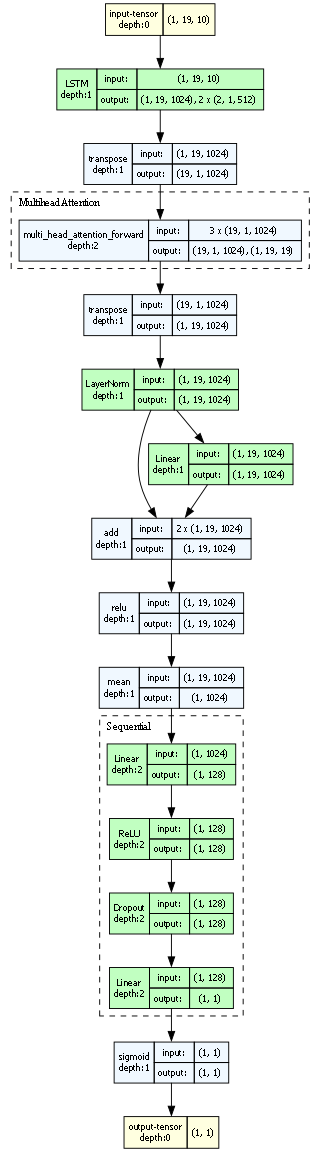
\includegraphics[width=0.4\textwidth]{figures/architecture.png}
  \caption[ResNet-BiLSTM-Attention Architecture]{ResNet-\gls{bilstm}-Attention architecture. Several layers are stacked, including \gls{bilstm}, residual connections, and attention mechanisms. The model processes input sequences, applies self-attention, and outputs a single value for binary classification.}
  \label{fig:architecture}
  \caption*{Source: Own Torchview illustration.}
\end{figure}

The architecture of the ResNet-\gls{bilstm}-Attention model is shown in \autoref{fig:architecture}. The \texttt{torch.nn} module integrates Bidirectional Long Short-Term Memory (\gls{bilstm}) layers with Multi-Head Self-Attention and Residual Connections. The model architecture consists of several layers, including convolutional layers, \gls{bilstm} layers, and attention mechanisms.

\begin{enumerate}
  \item \textbf{Input/Configuration:} The model is initialized with hyperparameters defining its structure: \texttt{input\_size} (number of input features, $D$), \texttt{hidden\_size} (dimensionality of \gls{lstm} states, $H$), \texttt{num\_layers} (number of stacked \gls{lstm}/Attention blocks, $N$), and \texttt{attention\_heads} (number of parallel attention heads, $A$).

  \item \textbf{\gls{bilstm} Layers:} The core consists of $N$ stacked \gls{bilstm} layers (\texttt{nn.LSTM} with \texttt{bidirectional=True}). Each layer processes the input sequence in both forward and backward directions, capturing dependencies from past and future context. The output dimensionality of each \gls{bilstm} layer is $2H$. Dropout is applied between layers for regularization.

  \item \textbf{Multi-Head Self-Attention:} Following each \gls{bilstm} layer, a \texttt{nn.MultiheadAttention} layer is applied. It performs self-attention on the \gls{bilstm} output sequence, allowing the model to weigh the importance of different time steps relative to each other within the sequence.

  \item \textbf{Layer Normalization \& Residual Connections:} \texttt{nn.LayerNorm} is applied after the attention mechanism within each block to stabilize activations. A residual connection adds the input to this block to the output before a final \texttt{ReLU} activation, facilitating gradient flow in deeper networks.

  \item \textbf{Sequence Pooling:} After the final \gls{lstm}/Attention block, the output sequence (shape: $Batch \times Sequence Length \times 2H$) is aggregated across the sequence dimension using temporal mean pooling (\texttt{torch.mean}), resulting in a single fixed-size vector (shape: $Batch \times 2H$) representing each input sequence.

  \item \textbf{Final Classifier:} A feed-forward network (\texttt{nn.Sequential}) processes the pooled representation. It typically includes one or more linear layers with \texttt{ReLU} activations and Dropout for regularization, culminating in a final linear layer producing a single output logit.

  \item \textbf{Output Activation:} A sigmoid function (\texttt{torch.sigmoid}) is applied to the final logit to produce a probability score between 0 and 1, suitable for binary classification. A threshold $\tau = 0.9$ discriminates the two classes (valid/invalid) during evaluation.

  \item \textbf{Weight Initialization:} Linear layers within the network are initialized using Kaiming Normal initialization (\texttt{nn.init.kaiming\_normal\_}), a standard practice often beneficial for layers followed by \texttt{ReLU} activations.
\end{enumerate}

For training, the model is set to training mode using \texttt{model.train()}. The model weights are updated using the \textit{\gls{adam}} optimizer \texttt{torch.optim.Adam} (\autoref{eq:adam}, \autocite{kingma2014adam}) with an initial learning rate of $0.001$. The loss function employed is binary cross-entropy (\texttt{nn.BCELoss}, \autoref{eq:bce}), which quantifies the difference between the predicted probabilities and the true binary labels. Input data is processed in sequences of length $19$. To prevent overfitting, dropout with a probability of $0.3$ is applied within the \gls{bilstm} layer and also in the final fully connected sequence. The \gls{bilstm} architecture itself consists of $1$ layer (\texttt{num\_layers=$1$}), with a hidden size of $512$ per direction (\texttt{hidden\_size=$512$}). A multi-head attention mechanism with $4$ attention heads (\texttt{attention\_heads=$4$}) is applied after the \gls{bilstm} layer. The final classification head uses an intermediate dense layer with $128$ units before the output neuron. See \autoref{sec:lstm} and following for a description of the theoretical background.

Instead of a fixed learning rate, a learning rate scheduler, specifically \textit{ReduceLROnPlateau} (\texttt{torch.optim.lr\_scheduler.ReduceLROnPlateau}), adjusts the rate during training. This scheduler monitors the training loss and reduces the learning rate by a factor of $0.1$ if the loss does not show improvement for $5$ consecutive epochs (\texttt{patience=$5$}). The model is trained for a default of $10$ epochs (\texttt{num\_epochs=$10$}), iterating over the training dataset in mini-batches of size $32$ (\texttt{batch\_size=$32$}), with shuffling enabled for the training data. In each epoch, the model performs forward and backward passes to compute the loss and gradients, subsequently updating the model parameters via the optimizer. The training loss is tracked per epoch to monitor convergence.

During evaluation (as seen in \texttt{evaluate\_model}), predicted probabilities are converted to binary labels using a threshold of $\tau = 0.9$. $\tau$ is chosen higher than the default because of the low tolerance for false positives (classifying simulated data as real) in the manufacturing context. Higher thresholds are commonly applied in anomaly detection or when the cost of a false positive is high. This value does not stand in contradiction to the rejection rate ($RR$) derived from the permutation testing (\autoref{sec:permtest}, \autoref{sec:model-logic}). The threshold of $0.9$ is a specific decision boundary for classifying individual instances post-training, impacting metrics like precision and recall at that specific cut-off point. In contrast, the permutation test assesses the overall statistical significance of the difference between the real and simulated data distributions, as captured by the model and features. It uses the \gls{roc} \gls{auc} score, which measures the models ability to distinguish between classes across \textit{all possible thresholds}, not just one. The rejection rate $RR$ then quantifies how consistently this statistically significant difference is found across multiple independent test runs. Therefore, a high $RR$ indicates that the model can reliably detect differences between real and simulated data, regardless of the specific threshold $0.9$ chosen for operational classification based on risk tolerance.

\section{Model Evaluation}
Based on the reference in \autoref{sec:metrics-theory}, the evaluation of the models is performed using various metrics. To achieve this, the model is switched to evaluation mode, \texttt{model.eval()}, to ensure deterministic behaviour. This disables dropout layers so that all neurons are used for the forward pass to achieve predictions. Gradient calculations are disabled through \texttt{torch.no\_grad()}. \texttt{BatchNorm} layers now use their learned estimates of mean and variance parameters to process the data. During evaluation mode, the model processes the test set batch by batch, yielding output probabilities. These are compared against the true labels. The evaluation metrics are implemented in the \texttt{evaluate\_model()} method. The evaluation metrics include a classification report, confusion matrix \autoref{tab:confusionmatrix}, accuracy \autoref{eq:accuracy}, precision \autoref{eq:precision}, recall \autoref{eq:recall}, F1-score \autoref{eq:F1-score} and \gls{roc} \gls{auc} score \autoref{eq:auc}. The metrics are calculated using the \texttt{sklearn.metrics} module. The evaluation metrics are used to compare the performance of the baseline model and the ResNet-\gls{bilstm}-Attention model as well as the standalone performance on the holdout set. The evaluation metrics are also used to diagnose the models and identify potential issues with respect to the bespoken adaptive feature selection procedure. For the assignment of the label 'valid' or 'invalid', a threshold $\tau$ of $0.9$ is used. This value is higher than the usual threshold of $0.5$. This means that if the predicted probability is greater than or equal to $\tau = 0.9$, the process execution is classified as 'valid'. If the predicted probability is less than $0.9$, the process execution is classified as 'invalid'. Setting the boundary so high is a conservative approach. It ensures that only the most confident predictions are classified as 'valid'. This is important for the \gls{vvuq} framework, as it aims to identify potential issues in the process execution. $\tau$ can be adjusted based on the specific requirements of the application and the desired trade-off between precision and recall.\footnote{For anomaly detection, setting $\tau$ higher is a common approach. In different contexts or sectors, lower thresholds may be better. A careful analysis of the \gls{roc} \gls{auc} curve may facilitate finding the best value.} The $0.9$ validity threshold reflects manufacturing \gls{vvuq}'s low tolerance for false positives \autoref{eq:precision}.